\chapter{Elementary number theory}
% TODO number theory missing concepts
% - (essential to proof of correctness of euclids algorithm)

% TODO extended missing concepts
% greatest common denomijator and least common muktiple

% - Newton's generalised binomial theorem
% - Add info about binominal theorem limitations (such as only integers)
% - Use binominal thorem to evaluate fractional powers
% - fundamental theorem of arithmetic: that every natural number greater than 1 is either prime,
% or else can be expressed as a product of primes in a way which is unique except for the order
% in which the primes are arranged.
% - the prime numbers are the basic building blocks from which all the natural numbers are constructed .
%% Fermat's Little Theorem
%% A number is divisible by another number (a divisor) if its prime factorization contains the prime factorization of the divisor. All numbers which divide such a number will have a factorization which is part of
%% Of particular interest in the non-negative integers i.e. elements of the set $\{0,1,2,3...\}}$, also known as the natural numbers and usually abbreviate as $\N$.
%% - phi and e are irrational
%% - prime counting function
%% - eliptic curves
%% - enhanced prime finding and locating algorihms (sqare root of n}
%% - one way functions and cryptography (RSA - the code book)
%% - Mesanine primes: Numbers that can be obtained by raising 2 to a power and then subtracting 1 are called Mersenne numbers, for reasons I’ll give later in the chapter. Prime numbers of this particular form are called Mersenne primes
% [BINOMAL]
%http://www.mcs.sdsmt.edu/ecorwin/finite_structures/bin_thm/bin_thm.html
%http://en.wikipedia.org/wiki/Binomial_theorem#Simple_derivation
%http://planetmath.org/encyclopedia/InductiveProofOfBinomialTheorem.html
%http://www.intmath.com/Series-binomial-theorem/4_Binomial-theorem.php
%http://www.matheclipse.org/en/Binomial_coefficient
%http://en.wikipedia.org/wiki/Binomial_coefficient#Combinatorial_interpretation

% https://en.wikipedia.org/wiki/Lindemann–Weierstrass_theorem#Transcendence_of_e_and_.CF.80 proof that pi and e and sin is not algebraic
% - http://planetmath.org/sites/default/files/texpdf/39438.pdf
% - http://www.math.brown.edu/~res/MathNotes/notes5.pdf
% - http://www.maths.bris.ac.uk/~malab/PDFs/MA469.pdf
% - https://www.math.leidenuniv.nl/scripties/BachWarrens.pdf

% primality tests http://math.stackexchange.com/questions/4597/simple-explanation-and-examples-of-the-miller-rabin-primality-test

% proof that e and pi is irrational then that they are trancedental

% Chinese remainder theorem http://en.m.wikipedia.org/wiki/Chinese_remainder_theorem

% Sieve of Eratosthenes algorithm impelementation

In number theory we deal with the properties of various classes of numbers such as the integers, which is any number that can be written without a fractional or decimal component and is denoted with the the symbol $\mathbb{Z}$. Thus,$-7$, $0$, and $2$ are integers; $1.7$ and $\frac{1}{7}$ are not. Incidentally the Latin word "integer" literally means "untouched", hence "whole". Of particular interests is the set of all positive integers, also known as the natural numbers and symbolised by $\mathbb{N}$.

\section{Basic properties of Integers}
Let us first consider that integers are either $even$ or $odd$, formally we write:
\begin{definition}\label{num_def}
The $even$ numbers are the numbers written on the form $2k$ and the $odd$ numbers are the numbers written on the form $2k+1$ where $k$ is any integer.
\end{definition}
some arithmetic can convince us that this indeed yields the desired numbers:
\[
\begin{array}{lcl}
2 \cdot 0     & = & 0 \\
2 \cdot 0 + 1 & = & 1 \\
2 \cdot 1     & = & 2 \\
2 \cdot 1 + 1 & = & 3 \\
:             &   & :
\end{array}
\]

The $odd$ numbers may also be expressed as being either one more than a
multiple of $4$ or three more than a multiple of $4$. Symbolically, we can say
that they are either of the form $4k + 1$ or of the form $4k  + 3$. Again some
examples clarifies the smoke
\[
\begin{array}{lcl}
4 \cdot 0 + 1 & = & 1 \\
4 \cdot 0 + 3 & = & 3 \\
4 \cdot 1 + 1 & = & 5 \\
4 \cdot 1 + 3 & = & 7 \\
:             &   & :
\end{array}
\]

incidentally this shows that when we divide a $odd$ number by $4$, we must get
a remainder of either $1$ or $3$ \label{remainder}. Armed with this knowledge
we can shine some light on the properties of $odd$ numbers:
\begin{corollary}
The square of an $odd$ number is $odd$
\end{corollary}
\begin{proof}
Consider, by \ref{num_def}, the algebraic form of the square of an odd number
\[
\begin{array}{lcl}
(2k+1)^2 & = & (2k)^2 + 2(2k) + 1 \\
                 & = & 4(k^2 + k) + 1
\end{array}
\]
The last expression being on the form $4k + 1$ yields the desired result.
\end{proof}

Integers can be used to construct another class of numbers, known as the rational numbers. Here we say a 'rational number' is a fraction $\frac{a}{b}$, where $a$ and $b$ are integers; we may suppose that $a$ and $b$ have no common factor (since if the had we could remove it) and that $b$ does not equal zero. We denote these numbers by $\mathbb{Q}$ for quotient. With only these properties at hand we can move on to prove one of mathematics first great results; that $\sqrt{2}$ is irrational.
\begin{proposition}
$\sqrt{2}$ is irrational.
\end{proposition}
\begin{proof}
To say that $\sqrt{2}$ is irrational is the same as saying $2$ cannot be expressed in the form $\left(\frac{a}{b}\right)^2$ or that the equation
\begin{equation}\label{2_irrational}
a^2 = 2b^2
\end{equation}
cannot be satisfied by integral values of $a$ and $b$ without any common factor. Let us for sake of eventual contradiction suppose that \ref{2_irrational} is true for some $a$ and $b$, then it follows that $a^2$ is even (since $2b^2$ is divisible by $2$) and thus that $a$ is even (since the square of an even number is even). If $a$ is even then
\[
a = 2c
\]
for some integral value of $c$; and therefore
\[
 a^2 = 2b^2 = (2c)^2 = 4c^2
\]
or
\[
b^2 = 2c^2
\]
Hence $b^2$ is also even and therefor $b$ is even. Now since both $a$ and $b$ are even they must have the common factor $2$. This contradicts our hypothesis, and therefore the hypothesis is false
\end{proof}
Notice how this proof is by \emph{reductio ad absurdum}, a proof style much beloved by the greeks and one of mathematics finest weapons. In these types of proofs we attack our theorem by taking an assumption and then show that it leads to a contradiction and hence is false.

\myindent Now since we have proved that $\sqrt{2}$ cannot be written as a fraction can we then find another way to express it ?. By definition, a number is $algebraic$ (denoted by $\mathbb{A}$) if it is the solution to some polynomial equation
\[
a_{n}x^{n} + a_{n-1}x^{n-1} + \cdots + a_{2}x^{2} + a_{1}x + a_0 = 0
\]
where all the coefficients $a_n, a_{n-1}, \cdots, a_2, a_1$ and $a_0$ are integers. Now as $\sqrt{2}$ is the solution to the polynomial $x^2 - 2 = 0$ it follows that it is a irrational algebraic number. Also as any integer $k$ is a solution to $x-k=0$ we see that all integers are algebraic and hence $\mathbb{Z} \in \mathbb{A}$. Later we shall meet another class of numbers known as transcendental numbers $\mathbb{T}$ which is simply the set of all non-algebraic numbers. As it turns  out almost all irrational numbers are transcendental and all transcendental numbers are irrational. The box below should hopefully clarify the relationships between these various sets of numbers
\begin{figure}[htb!]
\begin{center}
% TODO draw with tikz
%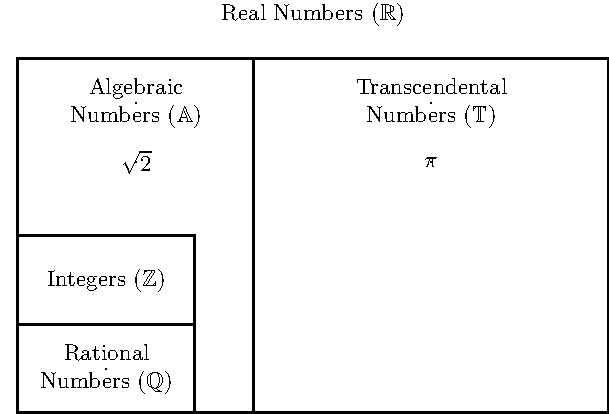
\includegraphics[width=10cm]{images/number_types.pdf}
\end{center}
\end{figure}
Note how all of these numbers are contained in the set of real numbers $\mathbb{R}$. The real numbers thus includes both integers and rational numbers, such as $42$ and $\frac{1}{3}$, and transcendental numbers, such as $\pi$ and irrational algebraic numbers such as $\sqrt{2}$. Informally we may think of real numbers as any number with or without a decimal point that may contain an infinite decimal tail that continue in some way.

\section{Divisibility}
The integer $n$ is divisible by $m$ if the ratio $n/m$ is an integer. Hence we write $m|n$ when $m$ divides $n$ evenly and define
\begin{equation}\label{divisibility}
m|n \Longleftrightarrow m > 0 \textnormal{ and } n = mk
\textnormal{ for some integer } k
\end{equation}

How do we know if a number is divisible by some other number ?. Here we are out of luck, in general we can only answer this by doing full division and checking if the remainder is zero. Mathematics contains many functions that are easy to do (such as multiplication and differentiation) but hard to undo (such as division and integration). Later on we will see that exactly this property of division can be used to craft a simple scheme for secure communication. For now let us extract some useful properties from the above definition of divisibility.
\begin{proposition}
If $a > b$ and $n$ divides $a$ and $b$ evenly then it also divide their
difference.
\end{proposition}
\begin{proof}
By \ref{divisibility} we have $a = nx$ and  $b = ny$ for some integral value of $x$ and $y$. Thus $a-b = nx - ny = n(x-y)$ as desired.
\end{proof}

As remarked on page \pageref{remainder} not all numbers divides evenly:
\begin{proposition}\label{division_algorithm}
If $a$ and $b$ are integers with $b\neq0$, then there is a unique pair of integers $q$ and $r$ such that
\[
a = qb+r \textnormal{ and } 0 \leq r \leq |b|
\]
\end{proposition}
Note that
\[
\frac{a}{b} = q + \frac{r}{b}
\]
where for $b>0$ we have $0 \leq \frac{r}{b} < 1$ and for $b<0$ we have $0 \geq \frac{r}{b} > -1$. As example the division $9/4$ with $a=9$ and $b=4$ becomes $9=2\cdot4 + 1$ giving us the quotient $q=2$ and remainder $r=1$
\begin{proof}
Our job is to prove that the numbers $q$ and $r$ exists, known as existence and that they are unique, also known as uniqueness. First we prove existence. Let
\[
S = \{a-nb|n \in \mathbb{Z}\} = {a,a \pm b,a \pm 2b,...}
\]
\end{proof}

\section{Euclid's Algorithm}
% GCD
The greatest common divisor of integers a and b, denoted by gcd(a,b), is the largest integer that divides (without remainder) both a and b. So, for example:

gcd(15, 5) = 5,	gcd(7, 9) = 1,	gcd(12, 9) = 3,	gcd(81, 57) = 3.

It is well known that if the gcd(a, b) = r then there exist integers p and s so that:

p(a) + s(b) = r.
By reversing the steps in the Euclidean Algorithm, it is possible to find these integers p and s. We shall do this with the above example:
Starting with the next to last line, we have:

3 = 9 -1(6)
From the line before that, we see that 6 = 24 - 2(9), so:
3 = 9 - 1(24 - 2(9)) = 3(9) - 1(24).
From the line before that, we have 9 = 57 - 2(24), so:
3 = 3( 57 - 2(24)) - 1(24) = 3(57) - 7(24).
And, from the line before that 24 = 81 - 1(57), giving us:
3 = 3(57) - 7( 81 - 1(57)) = 10(57) -7(81).
So we have found p = -7 and s = 10.

The procedure we have followed above is a bit messy because of all the back substitutions we have to make. It is possible to reduce the amount of computation involved in finding p and s by doing some auxillary computations as we go forward in the Euclidean algorithm (and no back substitutions will be necessary). This is known as the extended Euclidean Algorithm.

%http://www.math.utah.edu/~fguevara/ACCESS2013/Euclid.pdf
%http://pages.pacificcoast.net/~cazelais/222/xeuclid.pdf
Euclid devised a clever algorithm for locating the greatest common divisor.
% TODO GCD and LCM
% TODO add proof
\begin{algorithm}
    \caption{Euclid’s algorithm}
    \label{euclid}
    \begin{algorithmic}[1] % tells where the line numbering should start
        \Procedure{Euclid}{$a,b$} \Comment{The g.c.d. of a and b}
            \State $r\gets a \bmod b$
            \While{$r\not=0$} \Comment{We have the answer if r is 0}
                \State $a \gets b$
                \State $b \gets r$
                \State $r \gets a \bmod b$
            \EndWhile\label{euclidendwhile}
            \State \textbf{return} $b$\Comment{The gcd is b}
        \EndProcedure
    \end{algorithmic}
\end{algorithm}

\section{Primes}
A prime number is a natural number greater than 1 that cannot be formed by multiplying two smaller natural numbers. A natural number greater than 1 that is not prime is called a composite number. For example, $5$ is prime because the only ways of writing it as a product, $1 \cdot 5$ or $5 \cdot 1$. On the other hand $10$ is a composite as it can be written as $2 \cdot 5$. Semilarly 666 is not a prime as 
\[
666 = 2 \cdot 3 \cdot 3 \cdot 37
\]
 The first primes are
\[
2, 3, 5, 7, 11, 13, 17, 19, 23, 29, 31, 37 ...
\]
As we shall se later there are infintly many prime numbers. Prime numbers are thus important as they serve as the building blocks of other integers, indeed the following holds true:

\begin{proposition}\label{prim_div}
Every integer n $>$ 1 is divisible by at least one prime
\end{proposition}
\begin{proof}
Let $A$ be a composite number (i.e. non prime). By definition there must be some smaller number $B$ dividing evenly into $A$, where 1 $<$ $B < A$. Now either $B$ is prime or it is not. If $B$ is prime, then the original number $A$ indeed has a prime divisor, as claimed. Otherwise, $B$ is not prime and so has a divisor, say $C$, with $1 < C < B <$ A. If $C$ is prime, we are done, for $C$ divides evenly into $B$, and $B$ divides evenly into $A$. If $C$ is composite then it must have a proper divisor, $D$, and thus we continuously arrive at:
\[
A > B > C > D > ... > 1
\]
But all of these are positive integers, so we must reach a point in which we find a prime. Therefor any number, which is not prime itself, is divisible by at least one prime (usually, of cause, by several).
\end{proof}

If one surveys the list of the first 50 primes
\begin{lstlisting}
2, 3, 5, 7, 11, 13, 17, 19, 23, 29, 31, 37,
41, 43, 47, 53, 59, 61, 67, 71, 73, 79, 83,
89, 97, 101, 103, 107, 109, 113, 127, 131,
137, 139, 149, 151, 157, 163, 167, 173, 179,
181, 191, 193, 197, 199, 211, 223, 227, 229
\end{lstlisting}
then apparently the primes seams to be getting scarcer as the numbers go larger. Indeed between the numbers $1$ and $1000$ there are $168$ primes, whereas between $9000$ and $10.000$ there is but $112$. At first this seams logical enough since small numbers only have few possible factors and thus higher likelihood of being primes, yet one cannot help ask if we will ever reach such large numbers that the primes may eventually run out completely, rendering all subsequent numbers composite. Luckily this question had already been answered by the great greek mathematician Euclid who 300 B.C. in his IX book as proposition 20 indeed claimed:

\begin{proposition}
Prime numbers are more than any assigned multitude of prime numbers.
\end{proposition}
Euclid's terminology sounds strange, but what he is really proposing is that the sequence of primes does not end.
\begin{proof}
Let us for sake of eventual contradiction suppose that there is only a finite number of primes and that
\[
2, 3, 5, ..., P
\]
is the complete series (so that $P$ is the largest prime); and let us, on this hypothesis, consider the number $Q$ defined by the formula
\[
Q = (2 \cdot 3 \cdot 5 \cdots P) + 1
\]
It is plain that $Q$ is not divisible by any of $2, 3, 5, ..., P$; for it leaves the remainder $1$ when divided by any one of these numbers. But, if $Q$ is not prime, then by \ref{prim_div} it is divisible by some prime, and therefore there is a prime (which may be $Q$ itself) greater than any of them. This contradicts our hypothesis, that there is no prime greater than $P$; and therefore this hypothesis is false.
\end{proof}

Finding and counting primes is a long standing hobby for mathematicians, and one might ask if it can be automated. One such method was discovered by the greek mathematician Eratosthenes (ca. 284-192 B.C.) who as the chief librarian at the great Library at Alexandria spend much of his time studying mathematics, astronomy and philosophy. His method (known as Eratosthenes sieve) is as follows; write a list of all the consecutive integers, starting with $2$, among which you want to find the primes. As $2$ is prime, cross all subsequent multiples off. The next integer that has not yet been crossed of (3) must then also be prime and so we can eliminate all of its multiples. As we continue in this manner we will clearly sieve out all composite numbers and be left with the primes.
\begin{verse}\emph{
Sift the Twos and sift the Threes,\\
The Sieve of Eratosthenes.\\
When the multiples sublime,\\
The numbers that remain are Prime.}
\end{verse}
although this method will indeed generate the primes, it is not as efficient as one might have liked (although optimized and more complex methods exists). Later we shall encounter the prime counting function $\pi(n)$, which outputs the number of primes less than or equal to a given number $n$ (the use of $\pi$ in this function is an unfortunate standard as it has nothing to do with the well known geometric constant $3.1415...$).


\section{Modulo arithmetic}
% TODO missing modulo arithmetic
% - definition and excercises from http://www.math.rutgers.edu/~erowland/modulararithmetic.html
% - explain (perhaps in excercises) why the divisibility tests works
% - excercises
% --- sum of two even numbers is even
% --- the sum of an even and odd number is odd
% --- the product of two even numbers are even
As mentioned before integers can be broken up into the classes of even $..–6, –4, –2, 0, 2, 4, 6..$ and odd numbers $..–5, –3, –1, 1, 3, 5..$ There are certain generalisations we can make about the arithmetic of numbers based on which of these two classes they come from. For example, we know that the sum of two even numbers is even. The sum of an even number and an odd number is odd. The sum of two odd numbers is even. The product of two even numbers is even, etc.

Now we represent each of our two classes by a single symbol. We let the symbol "$0$" mean "the class of all even numbers" and the symbol "$1$" mean "the class of all odd numbers". The statement "the sum of two even numbers is even" can then be expressed by the following:
\[
0 + 0 \equiv 0 \textrm{ mod } 2.
\]
Here, the "$\equiv$" symbol is not equality but congruence, and the "$\textrm{mod} 2$" just signifies that our modulus is $2$. The above statement is read "Zero plus zero is congruent to zero, modulo two." The statement "the sum of an even number and an odd number is odd" is represented by
\[
0 + 1 \equiv 1 \textrm{ mod } 2.
\]
Those examples are natural enough. But when we try to express the statement "the sum of two odd numbers is even"? we get this strange looking expression
\[
1 + 1 \equiv 0 \textrm{ mod } 2.
\]
We have analogous statements for multiplication:
\begin{align*}
0 \cdot 0 &\equiv 0 \textrm{ mod } 2 \\
0 \cdot 1 &\equiv 0 \textrm{ mod } 2 \\
1 \cdot 1 &\equiv 1 \textrm{ mod } 2
\end{align*}
Basically we now have a number system with addition and multiplication but in which the only numbers that exist are 0 and 1. You may ask what use this has. Well, our number system is the system of integers modulo 2, and because of the previous six properties, any arithmetic done in the integers translates to arithmetic done in the integers modulo 2.

Since any integer solution of an equation reduces to a solution modulo 2, it follows that if there is no solution modulo 2, then there is no solution in integers. For example, assume that a is an integer solution to
\[
2a – 3 = 12,
\]
which reduces to
\[
0 \cdot a + 1 \equiv 0 \textrm{ mod } 2,
\]
or $1 \equiv 0 \textrm{ mod } 2$. This is a contradiction since no even number is an odd number. Therefore the above congruence has no solution, so a couldn't have been an integer. This proves that the equation $2a – 3 = 12$ has no integer solution.

\section{Exercises}
\begin{ExerciseList}

\Exercise What is the lowest number divisible by both $12$ and $20$
\Answer Numbers divisible by $12$ and $20$ also have to be divisible by each of their prime factors $12 = 2 \cdot 2 \cdot 3$ and $20 = 2 \cdot 2 \cdot 5$ thus $2 \cdot 2 \cdot 3 \cdot 5 = 60$.

\Exercise In 2000 the Jordanian mathematician, Murad A. AlDamen devised the following method for testing divisibility \pagenote{Found on the prime puzzlers project, at: \url{http://www.primepuzzles.net/puzzles/puzz_101.htm}}
\Question Use Murad's method to determine if $61$ divides $3598207$
\Question Prove Murad's method.
\Answer TODO
\end{ExerciseList}

\printpagenotes*


%Let L*M=N =n1+10n2, L(k1+10k2)=n1+10n2
%L*k1-n1=10a É.(1)
%-10Lk2=10a-10n2, Lk2=a-n2
%n2 ÐLk2=a É (2)
%add one to two and by N=M*L
%we find ((n1+10n2)(k1-k2)+ (k1+10k2)(nn-n1))/(k1+10k2)=11a, then (n2k1-k2n1)=0 (mod M)

% Divisibility rules excercieses
% http://mathforum.org/kb/message.jspa?messageID=1461184

% Binominal theorem excercises
% http://www.purplemath.com/modules/binomial2.htm

% GCF excercises
% Each time Miranda goes to the store she plans to spend $7, and each time Savannah goes to the store she plans to spend $9. A few weeks from now, Miranda and Savannah are surprised to find out that they have spent the exact same total amount of money at the store.
